\chapter{Introduction}\label{chapter:introduction}

Though cosmic rays were first discovered in 1912, their origins have to date remained a mystery. Since cosmic rays are charged particles and their paths through the universe are bent by magnetic fields, identifying the sources of cosmic rays is not as simple as tracing back their arrival directions at Earth. The discovery of the astrophysical neutrino flux in 2013~\cite{astroneutrinos} provides a new avenue for investigating this problem, as the sources of astrophysical neutrinos are suspected to be the same as high energy cosmic rays, but neutrinos are not charged, and thus their arrival directions point directly back to their source. Identifying the sources of astrophysical neutrinos (and consequently cosmic rays) would provide an entirely new view of the universe, potentially allowing us to examine regions opaque to more traditional astrophysical messengers such as photons. Additionally, neutrinos are a ``smoking gun" for hadronic acceleration, providing important information about the processes of particle production in astrophysical sources.

With the IceCube Neutrino Observatory having collected over 10 years of data, the first hints of astrophysical neutrino sources are beginning to be visible: a high energy alert event from the direction of the blazar TXS 0506+056 sparked multi-messenger followup that suggests neutrino emission from that location~\cite{TXS_Multimessenger}\cite{TXS_Archival}, and recent studies of time integrated neutrino emission from candidate blazars reveal a $3.5 \sigma$ excess of astrophysical neutrino events from the direction of the Seyfert II galaxy NGC 1068~\cite{10yr_tint}. 

These first hints of astrophysical neutrino sources raise several further questions: Could there be more sources like TXS 0506+056 or NGC 1068? How many? Is neutrino emission time-dependent, or steady? Perhaps most importantly, if there are more sources, how can we identify them? Though neutrinos are an excellent astrophysical messenger due to the correlation of their arrival directions with their source of origin, neutrino astronomy is made significantly more difficult by the existence of the atmospheric neutrino flux, which produces a large, irreducible background for searches of astrophysical neutrino sources. Because of this, high energy neutrino astronomy relies either on triggering off a multi-messenger signal (such as a blazar that was also detected in gamma rays), or leveraging knowledge about the pattern of neutrino emission (for example, the arrival directions of astrophysical neutrinos should be clustered near their sources of origin, while the atmospheric background should be isotropically distributed). 

This work will focus specifically on exploring the possibility of time-dependent neutrino emission, motivated in part by the archival followup that was performed by IceCube at the location of the blazar TXS 0506+056~\cite{TXS_Archival}. A novel method for fitting decorrelated ensembles of neutrino flare candidates is introduced and subsequently applied to source catalogs assembled according to properties of the TXS 0506+056 result that could potentially define a class of astrophysical neutrino sources. This new method of fitting ensembles of neutrino flares is intended to fill a methodological gap that exists in the field, as it provides a framework for combining (``stacking") neutrino flare candidates. 

This method is additionally applied to the entire neutrino sky, allowing for a more general examination of potential clustering of neutrino data in both space and time. If neutrino data is clustered beyond what is expected from the background hypothesis (isotropic arrival directions distributed uniformly in time), then that would be evidence of a population of astrophysical neutrino sources. Even in the case of a non-discovery, the method introduced here produces neutrino ``light-curves" (here referred to as ``flare curves") which are of potential use for future multi-messenger searches that may wish to incorporate information on historical neutrino emission from a particular source candidate.  

\begin{figure}[h]
\centering
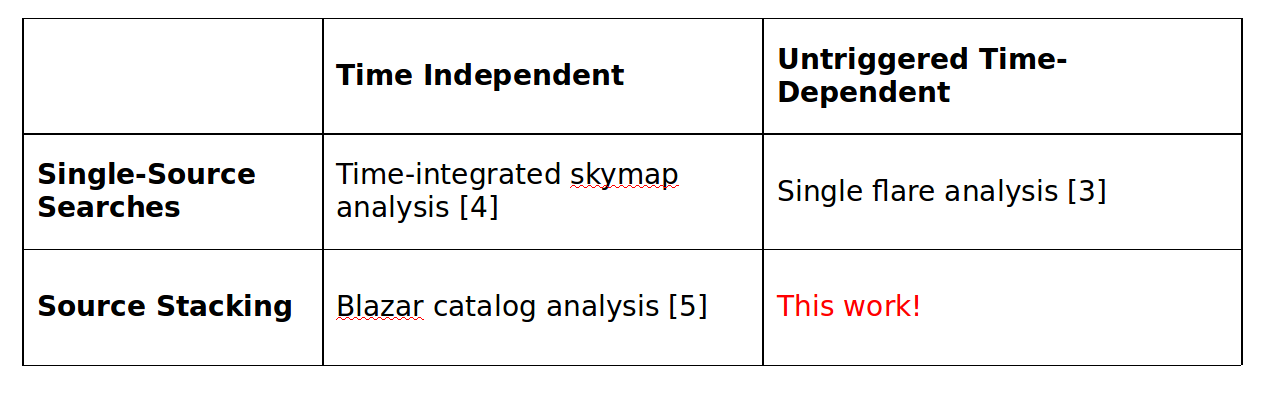
\includegraphics[width=0.9\textwidth]{figs/ana_table.png}
\caption{Examples of some of the types of astrophysical neutrino source searches that have been performed using IceCube data. Time-integrated analyses search for an excess of events over the entire data sample livetime, ignoring any information about potential temporal clustering. By contrast, untriggered, time-dependent searches attempt to fit for temporal neutrino clusters ("flares") without using a multi-messenger lightcurve as a template. Single source searches report the most significant result from a small number of source candidate locations, corrected by a trial factor, while source stacking analyses combine information from many source locations under the assumption that each source candidate is a weak emitter, thereby increasing the search sensitivity to low individual source flux. Note that this table is certainly not an exhaustive list of all types of neutrino source searches, as there are many other types of analyses that can be constructed (e.g. template searches, multi-messenger light-curve correlation analyses, cross correlation analyses~\cite{IC_HAWC_GP},~\cite{Fang_2020},~\cite{liu2021searching}). The analyses presented here are primarily intended to describe the space of analyses that are best suited for searching for point-like, flaring neutrino sources.}
\label{tab:anatable}
\end{figure}

This thesis is organized as follows:

\begin{itemize}
    \item Chapter 2 provides the scientific context and background information for this work, detailing the astrophysical messengers of interest (cosmic rays, photons, and neutrinos), their production mechanisms, and their relevance to modern multi-messenger astronomy. Several potential candidates of astrophysical neutrino sources are introduced, including TXS 0506+056 and NGC 1068.
    \item Chapter 3 describes the IceCube detector, which is used to collect the neutrino data used in the analyses presented later in this work. This section details both the physical components of the detector itself, as well as the triggering, event reconstruction, and data sample event selections that are relevant for the later chapters.
    \item Chapter 4 discusses the existing methods of untriggered searches for astrophysical neutrino flares, and subsequently introduces the new ``multi-flare" modification that is used to fit ensembles of flares at a candidate source location. This allows for a statistically efficient combination of the significance of multiple, sub-threshold flares, representing an improvement over previous methods that fit only the largest flare in the data sample.
    \item Chapter 5 presents the application of the multi-flare method to two source catalogs, motivated by previous results associated with the blazar TXS 0506+056. The first catalog is a catalog of 3LAC blazars detected by the Fermi LAT detector. The second catalog is formed by the locations of high energy IceCube events, in analog to the high energy alert event that triggered the follow-up of TXS 0506+056.
    \item Chapter 6 presents the application of the multi-flare algorithm on an all-sky scale, fitting for every potential neutrino flare candidate over the entire sky. Neutrino ``flare curves" at potentially interesting locations are examined, including the most significant multi-flare locations, as well as the previously discussed source candidates of TXs 0506+056 and NGC 1068.
    \item Chapter 7 discusses the outlook for neutrino astronomy, and places the results presented in this work in the context of the field as a whole. 
\end{itemize}

%\begin{table}[h!]
%\centering
% \begin{tabular}{||c c c||} 
% \hline
% . & Time-Integrated & Untriggered, Time-Dependent\\ [0.5ex] 
% \hline\hline
% Single Source & \cite{10yr_tint} & \cite{TXS_Archival} \\ 
% \hline
% Source Stacking & \cite{2lac_ic} & This work! \\
% \hline
%\end{tabular}
%\caption{Examples of some of the types of astrophysical neutrino source searches that have been performed using IceCube data. Time-integrated analyses search for an excess of events over the entire data sample livetime, ignoring any information about potential temporal clustering. By contrast, untriggered, time-dependent searches attempt to fit for temporal neutrino clusters ("flares") without using a multi-messenger lightcurve as a template. Single source searches report the most significant result from a small number of source candidate locations, corrected by a trial factor, while source stacking analyses combine information from many source locations under the assumption that each source candidate is a weak emitter, thereby increasing the search sensitivity to low individual source flux. }
%\label{tab:anatable}
%\end{table}



